\FloatBarrier
\subsection{Site selection}
\label{SiteInvestigation}
As described in the previous sections, ground motion may prove a limiting factor for the low frequency performance of ET. A preliminary site investigation was carried out to make a comparative analysis of various (underground) locations throughout Europe and across the globe. The following paragraphs will discuss the measurement procedures and a list of locations that have undergone investigation. In order to ascertain all site characterisation procedures were carried according to seismologic standards, measurements and data collection was carried out partly in collaboration with the Observatories and Research Facilities for European Seismology (ORFEUS) which is maintained by seismology department of the Royal Netherlands Meteorological Institute (KNMI). Measurements from all locations were obtained over a two month period to ensure minimal seasonal variations. 

In order to measure the ambient seismic background low noise broadband seismometers are required. All seismic measurements were carried out using two measurement stations, each station consists of a Trillium 240 (T240) accelerometer and a data acquisition system. The T240 is a broadband low noise seismometer with a flat velocity response from 4 mHz to 35 Hz and a self noise below the low noise model from 0.01 to 10 Hz. The on-site seismic measurements were made over a period of 5 to 6 days. Care was taken to ensure that the measurement time includes at least a weekend and a number of week days. 

The following includes an summary and results from selected locations. In all of the following results a fast Fourier transform (FFT) was performed on stretches of 128 seconds of data to obtain an power spectral density (PSD) in (m$^2$/s$^4$)/Hz. The PSDs are averaged over a period of half an hour. Averaged PSD values are smoothed by taking the average of the PSD values in a constant relative bandwidth of 1/10 decade. (So for low frequencies the averaging is over only a few points, for high frequencies the averaging is over many more points). For comparison the new high and low noise models are also plotted. Spectral variation plots are used here to not only show the amplitude of the seismic signal but also how much time, as a percentage, is spent at a certain level. This is indicated by the color of the plot. The spectral variation plots also contain three solid line plots to indicate the mode and the 90 and 10~\% levels. The mode is the most common PSD value in each frequency bin, and 90 and 10~\% levels indicate the point under which the PSD will stay for 90 or 10~\% of the time, respectively. 

\FloatBarrier
\subsubsection{Measurement sites}
The following section provides a brief description of all locations included within the site characterization and classification program. The selection criteria for these sites was based on the availability of a suitable underground measuring location. Gaining safe access to underground locations with little or no nearby (underground) activity proved very challenging. The majority of the sites are therefore already existing underground laboratories or decommissioned mines that are undergoing environmental rehabilitation or being converted for tourist purposes. Initial selection procedures were based on general suitability for a GW telescope and surface measurement of seismic data. The main purpose of this research was to ear-mark 3 or 4 locations for an extensive seismic and geological study. A followup site selection study would address in more detail the suitability of constructing the Einstein Telescope observatory at or near the location or in similar geological conditions.  

A brief description of each location will now be given, followed by a more detailed summary of a selection of sites. The position of each site is displayed on a map given in Fig.~\ref{Fig:map}.

\begin{figure}[h]
	\begin{center}
		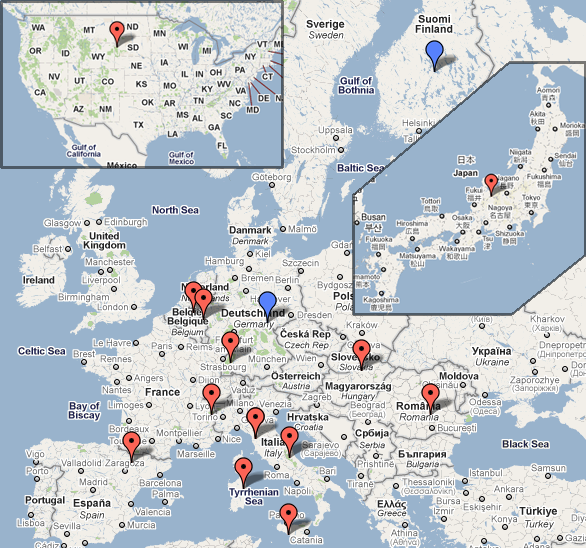
\includegraphics[width=0.65\textwidth]{./Sec_SiteInfra/Figures/map2.png}\hspace{1pc}%
		\caption{Map displaying position of the seismic measurement sites presented in this report. Red icons with a dot indicate locations where measurements were taken at underground locations, blue icons indicate where data were obtained via the Orfeus network from surface installations.}
		\label{Fig:map}
	\end{center}
\end{figure}

\begin{itemize}

\item \emph{The Netherlands: Heimansgroeve.}
The Heimansgroeve is an old quarry situated in the very southern tip of the Netherlands. It contains the oldest rock type found in the Netherlands, Carboniferious, about 360 - 300 million years old. The stone consists of slate and carbonic sandstone. The Royal Netherlands Meteorological Institute has a seismic observatory in a small underground laboratory some 10 meters below the surface. Our seismic stations were placed alongside the institutes permanent seismometers which provided an excellent cross check between instruments and analysis.

\item \emph{Hungary: Gy\"ongy\"osoroszi.}
The Gy\"ongy\"osoroszi mine is situated some 107 km North-East from Budapest in the M\'atra mountains. This old zinc-lead mine has horizontal access with underground depths ranging from 100 to 350 m at an elevation of about 400 m. Local rock type consists of andezit and andezit tufa. A ecological rehabilitation of the neighourhood and mine was started last year. The mine contains a number of long straight drifts of which the longest is 3 km. The seismic stations were placed 1.4 and 3.8 km from the entrance at depths of 70 and 400 m respectively. There is a permanent Seismological Observatory of the Hungarian Academy of Sciences at Piszk\'estet\"o on the site of the Konkoly Thege Astronomical Observatory. It is situated about 4 km from the mine entrance.

\item \emph{Romania: Slanic.}
Slanic-Prahova is located, 40 km NE of Ploiesti, or 100 km north of Bucarest in Romania. Very large caverns 30 m wide and 35 m high, dug in salt, are presently existing and a low background laboratory was successfully installed in one of the caverns. The salt exploitation ended in 1971, however another salt mine is still active in the same salt deposit. For the time being the mine is used for tourism and medical purposes. Access into the mine is available via an elevator able to carry up to 10 tons. The network of galleries of Unirea salt mine is very large. The current area is 70 000 m$^2$ with 2.9 million m$^3$ having already been excavated. Nearby seismic stations show very low seismic activity in the area. Both seismometers were set-up side by side at a depth of 190 m.

\item \emph{France: Frejus.}
The underground laboratory LSM `Laboratoire Souterrain de Modane', is located along the road tunnel between the French Modane and Italy. The overburden at this site is 1700 m of hard-rock or 4800 meters of water equivalent. The LSM, in operation since 1982, already hosts two particle physics experiments requiring an extremely low-background environment to study neutrino properties and to search for dark matter. A seismic station was set-up next to a large neutrino experiment.

\item \emph{Spain: Canfranc.}
The Canfranc Underground Laboratory (LSC, `Laboratorio Subterr\'aneo de Canfranc') is located on the Spanish side of the Pyrenees, under the mountain of `El Tobazo' and has various particle physics programs aimed at very low background experiments for the study of neutrino properties and the search for dark matter. It has 2500 m water equivalent overburden at depths of around 900 m and can be accessed via the roadway or decommissioned railway tunnels.

\item \emph{Italy: Gran Sasso.}
The Gran Sasso National Laboratory is the largest underground laboratory in the world for experiments in particle physics, particle astrophysics and nuclear astrophysics. It is located between the towns of L'Aquila and Teramo, about 120 km from Rome. The underground facilities are located on one side of the ten kilometer long freeway tunnel through the Gran Sasso Mountain at an average depth of 1400 m. They consist of three large experimental halls, each about 100 m long, 20 m wide and 18 m high and service tunnels, for a total volume of about 180,000 m$^3$. A seismic station was placed in an escape gallery between the road and railway tunnels at a depth of 800 m.

\item \emph{Italy: Sardinia.}
The Mediterranean island of Sardinia is seismically quieter than the Italian main land. This is due to its more central position on the European tectonic plate, as opposed to near its boundary. Measurements were performed in a mine near Lula, 50 km south of Olbia on the north-eastern side of the island. This former lead-zinc mine is currently being rehabilitated to allow safe passage into the mine for tourists. 

\item \emph{Italy: Sicilie.}
The Italkali salt mine is situated near the town of Realmonte on the southern coast of Sicily, 10 km east of Agrigento. Salt is excavated by creating huge caverns, some as large as 100 m in length. Measurements were taken at a depth of about 60 m, at an elevation of 30 below sea level. Both stations were installed in a storage cavern about 50 meters apart. One seismic station was on a large concrete pad with the other was placed straight onto the salt floor. The mine was still in active use with a nearby conveyor belt in continuous operation during the measurements. 

\item \emph{Germany: Black Forest.}
The Black forest observatory (BFO) is a geophysical observatory in operation since 1972, owned and operated by Karlsruhe University and Stuttgart University. It is located in an abandoned silver mine and contains gravimeter, seismometers, tiltmeters as well as electromagnetic and weather sensors. The local rock type is granite and the overburden is up to 180 m. The measurements were taken at a depth of 90 m along side of the BFO.

\item \emph{Finland: Sumiainen.}
The Finish bedrock is amongst the oldest and most stable in Europe, ranging from 3.5 to 2.6 billion years old, making it cheap and relatively trivial to construct underground caverns and tunnels. For this reason much of the infrastructure in Finish cities is built underground. Finland's isolation from major oceans and small population density could prove ideal for a low seismic background environment. No site was visited but data from an already installed surface seismic observatory in central Finland, near Sumiainen, was acquired.

\item \emph{Belgium: Mol}
Near Mol in northern Belgium an underground laboratory has been constructed to investigate the long-term effects of construction in the "Boomse" clay layer. Clay is impenetrable to water and has self healing properties. For these reasons it has been proposed as an excellent candidate for the long-term storage of highly active nuclear waste. The HADES underground laboratory administered by EURIDICE is situated at a depth of 230 m in a clay layer roughly 150 m thick. In 2002 a new gallery was constructed, in a cylindrical form with a diameter of 4 m and a length of 80 m. A seismic station was setup in the new gallery and measurements were taken during the Christmas break of 2010.

\item \emph{Japan: Kamioka}
CLIO, a 100 m prototype cryogenic gravitational wave detector has successfully been built in the former Kamioka mine near Toyama, 200 km west of Tokyo. The same mine is also home to the Super-Kamiokande neutrino observatory, and, in the future, will house the 3 km Large Cryogenic Gravitational Telescope (LCGT). Two seismic stations were installed at the CLIO end stations at depths of around 1000 m.

\item \emph{USA: Homestake}
The Homestake mine is located in Lead near the western border of the state of South Dakota. Until its closure in 2002 it was the largest and deepest gold mine in North America. It is also famous for the deep underground experiment, set up by Raymond Davis Jr., that was the first to detect solar neutrinos. Since 2007 the mine is being rehabilitated to house the Deep Underground Science and Engineering Laboratory (DUSEL). An array of seismic stations is being installed at depths ranging from 0 to 1500~m and will be the first of its kind in terms of 3D coverage and depth. Two seismometers have been contributed to this array and data were taken for several months in 2010.

For comparison, data were also taken at Virgo detector in Italy, the GEO detector in Germany, and the Kamioka mine in Japan.

\end{itemize}


%%%%%%%%%%%%%%%%%%%%%%%%%%%%%
%		 sites
%%%%%%%%%%%%%%%%%%%%%%%%%%%%%./Sec_SiteInfra/Figures
\FloatBarrier
\subsubsection{Results from a selection of sites}
The following section discusses, in some more detail, three sites that have been selected for further investigation. A complete list of measurements and results is located in Appendix B.1. Seismic measurement results will be presented and discussed, then summarized in the following section. 
\FloatBarrier
\subsubsection*{Sos Enattos mine, Sardinia, Italy}
The Sos Enattos mine, Lula, Sardinia, is a former lead and zinc mine of schist rocks composed of sphalerite ([Zn,Fe]S) and galena (PbS). It is situated 50 km south of Olbia on the north-eastern side of the island, 20\,km from the coast. A map of the mine is shown in Fig~\ref{fig:sosenattos}, where the yellow circle indicates the experimental area where the measurements were carried out. The seismometers were placed at a depth of 189 m, at an elevation of 206 m above sea level. Data were collected from June 31, to July 5, 2010. The most significant plots, obtained by applying the analysis method described in a previous section, will be presented here.

\begin{figure}[h]
	\begin{center}
		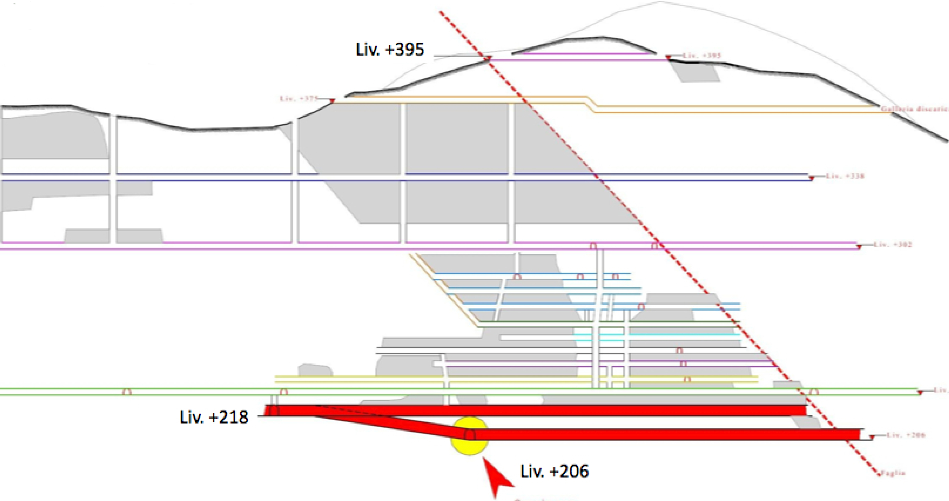
\includegraphics[width=0.9\textwidth]{./Sec_SiteInfra/Figures/sosenattos2.pdf}
		\caption{Underground map of the Sos Enattos mine, Sardinia. The yellow spot indicates the measurement location, at an elevation of 206 m and depth of 189 m.}
		\label{fig:sosenattos}
	\end{center}
\end{figure}
The spectral variation plots from data taken from the Sos Enattos mine are shown in Fig. \ref{fig:Lula-A_multiplot1}. The primary and secondary microseismic peaks are visible at 0.08 and 0.2 Hz respectively and are within an order of magnitude or touching the low noise model. This is due to the relatively large distance to the Atlantic ocean (1000 km to west coast of France). At higher frequencies, between 0.4 and 0.8 Hz an extra 'tertiary' microseismic peak can be seen. This is due to similar effects that cause the primary and secondary micro-seismics but originate from the Mediterranean sea and are typical of other Italian sites~\cite{marchetti}.

In the frequency range from 2 to 20 Hz a large variation in the spectral density is evident. Observing the spectrograms in Fig. \ref{fig:Lula-A_multiplot2}, that plot the spectral density as a function of time it is clear to see that this variation has a daily pattern, indicating that the seismic noise sources at these frequencies originate from anthropogenic sources. More over, in the 2 - 8 Hz range the heightened activity seems to occur during the late morning hours before noon, on all days except Sunday. This coincides with the miners schedule of underground works and tourist activity during these hours. 
\begin{figure}[h]
	\begin{center}
		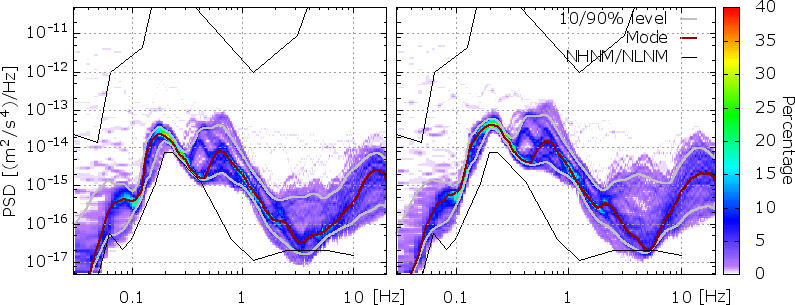
\includegraphics[width= 0.8\textwidth]{./Sec_SiteInfra/Figures/Lula-A_multiplot1}
		\caption{The horizontal component (left) and the vertical component (right) power spectral density plotted as a spectral variation from the Italy - Sardinia site. The 'tertiary' microseismic peak as a result of microseismics from the Mediterranean sea is evident from 0.4 to 0.8 Hz. Large variations at higher frequency are a result of work in the mine and other anthropogenic activity.}
		\label{fig:Lula-A_multiplot1}
	\end{center}
\end{figure}

\begin{figure}[h]	
	\begin{center}
		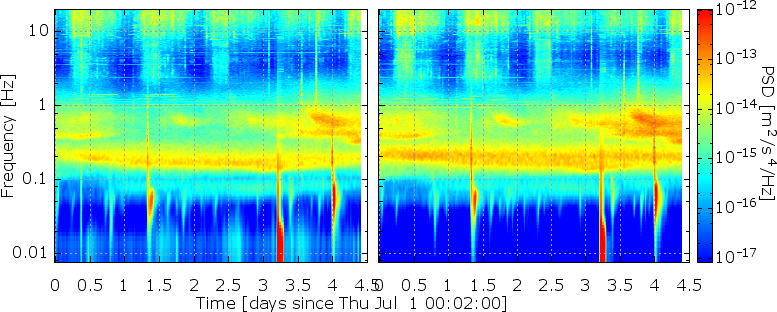
\includegraphics[width= 0.8\textwidth]{./Sec_SiteInfra/Figures/Lula-A_multiplot2}
		\caption{The spectrogram of the horizontal (left) and vertical (right) component from the Italy - Sardinia site. Day and night variation is visible as is the morning underground activity on Thursday, Friday and Saturday.}
		\label{fig:Lula-A_multiplot2}
	\end{center}
\end{figure}

\subsubsection*{LSC, Canfranc, Spain}
\label{sec:spain}
The Canfranc Underground Laboratory is located under the mountain 'El Tobazo' in the Northern Pyrenees, along the 8.5 km road tunnel spanning the French-Spanish border. Situated under 850 m of rock providing an overburden a 2500 m water equivalent makes it suitable for low background experiments. Access to the laboratory is via either the road tunnel or a parallel decommissioned railway tunnel. 

Seismic measurement stations were set up at two separate locations. The first was just behind the access door to a small low background laboratory along the railway tunnel. Due to continuous mechanical activity from pumps and ventilators in the laboratory as well as near-by construction work at the main laboratory, the data from this station were deemed unsuitable for background seismic measurements. A second seismometer was installed in a gallery connecting the road and railway tunnels and acts as an emergency escape route. This location was half way along the tunnel and 1 km away from the laboratory and other human or mechanical activity (besides the traffic in the road tunnel, 50 m away) at a depth of 900 m. 

\begin{figure}[h]
	\begin{center}
		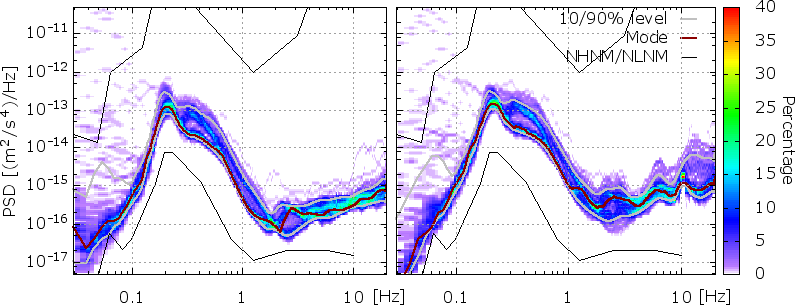
\includegraphics[width=0.8\textwidth]{./Sec_SiteInfra/Figures/Canfranc-B_multiplot1}
		\caption{The horizontal component (left) and the vertical component (right) power spectral density plotted as a spectral variation from the Spain - Canfranc Underground Laboratory site. The large microseismic peak is a result of the sites proximity to the Atlantic ocean. The small spectral variation at high frequencies is due to the low population density of the area.}
		\label{Canfranc-B1}
		\end{center}
\end{figure}

\begin{figure}[h]
	\begin{center}
		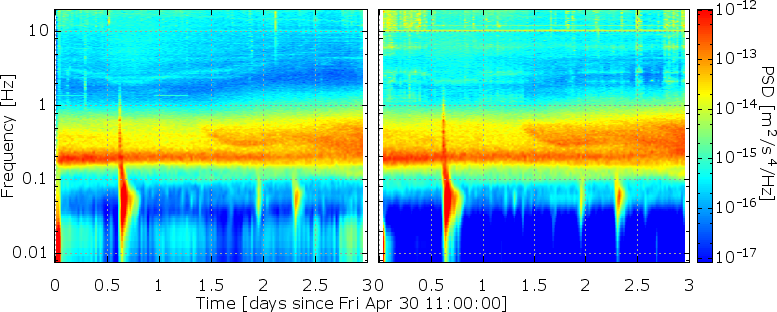
\includegraphics[width=0.8\textwidth]{./Sec_SiteInfra/Figures/Canfranc-B_multiplot2}
		\caption{The spectrogram of the horizontal (left) and vertical (right) component from the Spain - Canfranc Underground Laboratory site. No difference in day and night activity is distinguishable indicating there are no anthropogenic sources contributing to seismicity at this site. }
		\label{Canfranc-B2}
	\end{center}
\end{figure}

The results from the second Canfranc seismic station are shown in Fig.~\ref{Canfranc-B1} in the form of spectral variation plots. The high microseismic peak around 0.2 Hz is evident consistent with the relatively close proximity of 130 km to the Atlantic ocean. At higher frequencies (2 - 20 Hz), where seismic noise is predominantly a result of anthropogenic noise, the seismicity is low. The variation in the PSD values at these frequencies is low, having just half an order of magnitude between the 10 and 90 \% levels. In the spectrograms in Fig.~\ref{Canfranc-B2}, the day and night variation, a measure of anthropogenic activity, is not observed, a result of the very low population density of the area and the considerable depth of the site. This was also evident in day and night ratios, plotted in Fig.~\ref{fig3.3}, of this and the other sites presented in this section.
 
\FloatBarrier
\subsubsection*{Gy\"ongy\"osoroszi mine, Hungary}
\begin{figure}[t]
	\begin{center}
		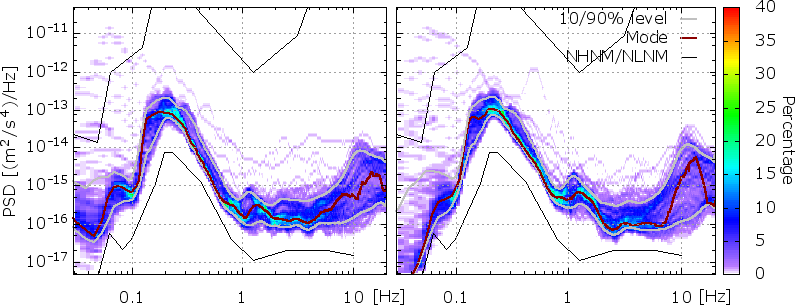
\includegraphics[width=0.8\textwidth]{./Sec_SiteInfra/Figures/Hung-A_multiplot1}
		\caption{The horizontal component (left) and the vertical component (right) power spectral density plotted as a spectral variation from the Hungary - Gy\"ongy\"osoroszi mine site. The microseismic peak drops off quickly providing a low noise at 1 Hz. Large spectral variation at higher frequencies is due to anthropogenic activity.}
		\label{fig:Hung-A_multiplot1}
		\end{center}
\end{figure}

The Gy\"ongy\"osoroszi mine in Hungary is a former lead and zinc mine that is currently being rehabilitated for environmental reasons. This provided an excellent opportunity to enter safely into the mine without any large scale mining activity nearby. It is situated 107 km north-east of Budapest in the M\'atra mountains at an elevation of 400 m above sea level. The surrounding geology is Andezite. Access into the mine was possible on an electric locomotive through a horizontal access tunnel. 
\begin{figure}[h!]
	\begin{center}
		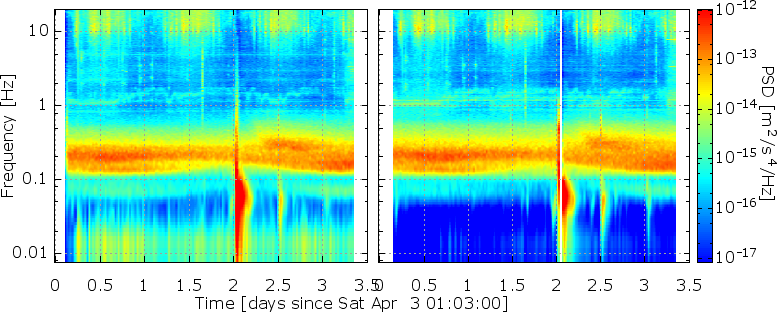
\includegraphics[width=0.8\textwidth]{./Sec_SiteInfra/Figures/Hung-A_multiplot2}
		\caption{The spectrogram of the horizontal (left) and vertical (right) component from the Hungary - Gy\"ongy\"osoroszi mine site. The large event after 2 days is an Earthquake in Mexico with a magnitude of 7.2. Day and night variations due to anthropogenic noise at higher frequencies is still visible.}
		\label{fig:Hung-A_multiplot2}
	\end{center}
\end{figure}

Two separate seismometer stations were installed at locations along the main drift. At each site the miners had excavated a small hollow into the tunnel wall so that the instruments could be safely installed without being inundated by the small, but steady, flow of water and mud. The first location was 1435 m from the entrance with a rock overburden of 70 m. The second location was 3750 m from the entrance at a depth of 400 m. A permanent seismic station of the Hungarian Academy of Science was situated at the surface, just 2.5 km away from the deepest station. Data were also obtained from this station and compared with the two underground sites. The results were presented in Fig.~\ref{fig3.6} and show an order of magnitude decrease in seismic noise between the surface and underground locations at frequencies above 1 Hz. 

The spectral variation plot of the Gy\"ongy\"osoroszi seismic results are plotted in Fig.~\ref{fig:Hung-A_multiplot1}. The microseismic peak at 0.2 Hz is again obvious and its tail drops off faster than, for example, the Spanish site. From 1 to 8 Hz the acceleration PSD of the horizontal component stays flat and just 1.5 orders of magnitude above the NLNM. At higher frequencies the upper limit of the spectral variation increases by another order of magnitude. This is due to anthropogenic activity that is penetrating down to the measurement site. Evidence of this can be seen in the spectrogram plotted in Fig.~\ref{fig:Hung-A_multiplot2}, where a clear day and night pattern is visible.

\pagebreak

\FloatBarrier
\etbox{r}{box:site}
{Site selection summary}
{The preliminary site investigation set out to explore the possibilities of finding a suitably seismically quiet environment for ET. Seismic measurements were taken at several sites throughout Europe and data were also analyzed from a number of existing seismic observatories. A complete list of measurement results is located in Appendix B.1. It has been shown that at a number of sites visited the seismic background environments is comparable to that for LCGT. The spectral variations were taken over periods of a week. Three sites where selected according to their seismic suitability and presented here. The results of these underground sites, the near surface site in the Netherlands and from the site of the existing GW detector Virgo, are plotted for comparison in Fig.~\ref{fig:sitecomparison}. It is clear to see that moving to a quiet location can improve seismic noise effects by several orders of magnitude. In the case of the underground sites by comparison to the Virgo site, up to 5 orders of magnitude improvement in terms of seismic acceleration power can be obtained. A follow-on study is proposed at, or in similar geographical conditions to, these sites to investigate long-term seismic and geological characteristics and investigate the possibility of housing large underground facilities. 
\begin{figure}[H]
\centering
	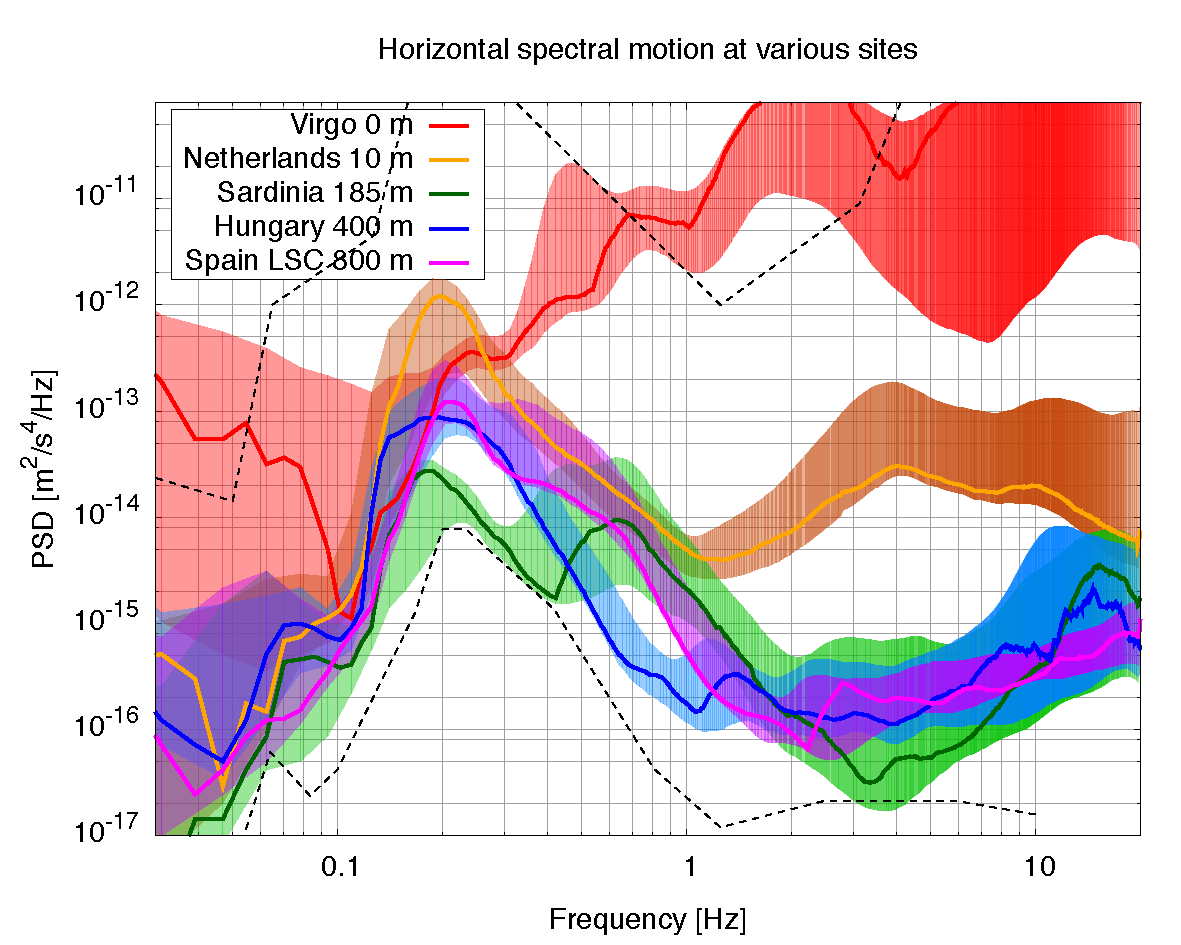
\includegraphics[width=0.95\textwidth]{./Sec_SiteInfra/Figures/BestSiteComparison.pdf}
	\vskip 0.3cm
	\caption{One-week spectral variation results of the three European sites. Plotted for comparison is the site of the current GW detector Virgo. The solid lines correspond to the mode, while the upper and lower limits of the transparent regions are the PSD levels that weren't exceeded for 90 and 10 \% of the time respectively.}
	\label{fig:sitecomparison}
	\end{figure}
}
